\section{Improving IE for the Future}

The goal of this paper has been to show some of the weaknesses of current approaches to information ecology and propose some potential areas where information ecology can become more fruitful. This section of the paper discusses some of the potential areas where IE could become even more influential in the information sciences.

One of the key confusions between the term "information ecology" and the research program carried out so far under that rubric has been the matter of how ecological concepts are adapted by a field that is far from the biological origins of the first concepts. Our critiques pose a number of questions of just how far the ecological metaphor can be applied to information and technical systems created and maintained by human beings. One value of an ecological perspective is realizing that human created systems are connected to the environment and cannot be separated from nature [and we cannot forget these roots]. Many of the thinkers who have been attracted to the concept of information ecology are deeply concerned about the environmental impact of human activity and the role of information and communication technologies in perpetuating and sometimes exacerbating those impacts. The growing demands for the information technology industry to acknowledge the environmental impact along the entire product chain from the mining of rare earth minerals, to the costs of energy production, to the final disposal of electronic waste is an indication that an ecological perspective is critical to the future of information science (see figure 4.). The idea of big data as a form of information pollution is another question posed by an ecological critique of information systems. Environmental and social impacts of technology need to be considered across scales from the micro impact of an electronic disposal plan through to the social impact of big data.

\begin{figure}[!ht]
  \centering
    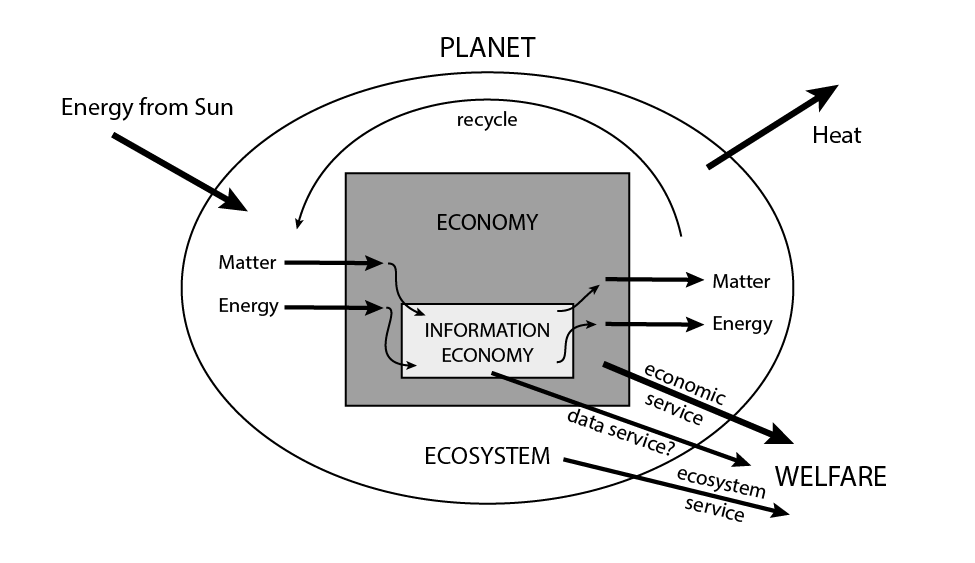
\includegraphics[width=1.0\textwidth]{figures/EcolEcon}
  \caption{The information economy understood as a sector of the global economy which itself is a sub-system of the global ecosystem. This vision comes from ecological economics which is a project to turn the classical economic vision of the ecosystem as a part of the economy to the reverse, the eonomy is a part fo the ecosystem. In a similar manner the information economy, data assemblages, or whatever name we choose, is also a part of the ecosystem an cannot be an ecosystem or ecology itself. Adapted from \citep[][p. 18]{daly_2004}}
\end{figure}

How can we expand the current discussion of information ecology to make it more powerful for the future. We propose the following areas for improvement

\subsection{Deepening the Information Eco- Theory}

The seeds for information ecology have been germinating for over 30 years. Now is the time to encourage their growth and one way to do that is to take seriously the parallels between information systems and the ecological systems from which we seek to borrow ideas. Too many of the ideas imported from ecology into information science have been adopted at a superficial level. Those ideas need to be developed more fully and clearer differences established between human and natural systems [note: this language choice is poor and needs to be worked on]

Questions about information diffusion, sharing, and communication will benefit from a deeper examination of how ecological thought may impact those parts of the information ecosystem. One of the areas where information ecology ideas have gained a foothold is in the management information systems literature. Up to this point many of these studies have focused on evaluating information systems in order to improve business processes. Information ecology could also benefit from greater international participation, especially in developing countries. \citep{wang_information_2015}

\subsection{Random thoughts}

Engage with dynamic socio-ecological systems research \citep{liu_etal_2007}.

Follow the example found in the information ecology literature that studies the Long Term Ecological Research network and their data management practices. In the Baker and Bowker article entitled "Information Ecology: open system environment for data, memories, and knowing" the authors engage deeply with information ecology from the management perspective outlined by DP, but are very careful to refer only to natural ecosystems and to distinguish them from what they term "digitally constructed memories" or "cross-domain knowledge bases" that comprise global collections of data/information about ecosystems \citep[][p. 131]{baker_2007}.

Be wary of the confusion of ecology with ecosystems \citep[cf. ][]{lucas_2012,nardi_information_1999}. Although much like economy has two meanings--the study of economic systems and the economic system itself--perhaps ecology will be the same someday (see OED, can be the study of the relationships or the relationships themselves)? But note, a common conception of the economy is that it draws material wealth from nature--stocks and flows of natural resources, minerals, water, energy and so on. Then value-added modifications are made to the resources and the resulting products are exchanged in human created markets for either use, consumption, or aesthetic purposes. Finally the waste streams from the economic activity are then returned to nature. In other words the economy is entirely dependent on nature and indeed is a human-created subsystem of natural processes. An ecosystem or ecology, on the other hand, is an abstraction of nature and the relationships between living organisms and their surrounding non-living environment. While living organisms, including humans, have a dialectical relationship with ecosystems--organisms influence the ecosystem and the ecosystem influences organisms--an ecosystem is not purposefully made by the organisms for exchange [or is it??]. Once again we are back to the third and most difficult question that humans have grappled with when analyzing their relationship with nature. Does nature have purpose? To reduce an ecosystem to human-made, such as an information ecosystem, denies possibilites of spiritualism and non-quantifiable relationships that we have with nature.
